\section{shapes and fonts: examples}

\begin{figure}
	\centering
	\includegraphics[width=4in]{figures/shapes/rlc.png}
	\caption[RLC]
	{RLC circuit.}
\end{figure}

\begin{figure}
	\centering
	\includegraphics[width=4in]{figures/shapes/rcline.png}
	\caption[RCline]
	{RC line circuit.}
\end{figure}


\begin{figure}
	\centering
	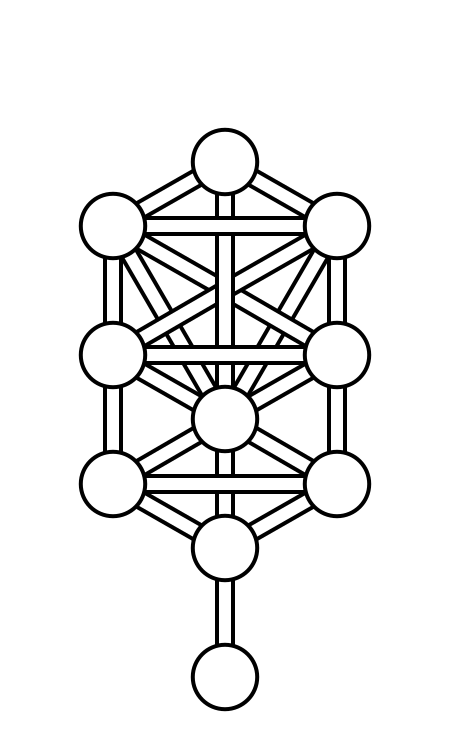
\includegraphics[width=4in]{figures/shapes/treeoflife.png}
	\caption[treeoflife]
	{The Tree of Life from Jewish mysticism.}
\end{figure}

\begin{figure}
	\centering
	\includegraphics[width=4in]{figures/shapes/treeoflifespelling.png}
	\caption[treeoflifespelling]
	{Symbol glyph spelling of Tree of Life. What makes things like this easy to make is building up building blocks like the cross pieces of all different scales, and the use of universal symmetries and scales(6 fold, 12 fold, and the square root of 3 and 2).}
\end{figure}

\begin{figure}
	\centering
	\includegraphics[width=4in]{figures/shapes/estrogendiagram.png}
	\caption[estrogendiagram]
	{Molecular symbol for the steroid hormone estrogen.  Note the characteristic hexagon-pentagon combination which is repeated throughout self-replicating chemical systems(life) as well as throughout the Geometron system/language.}
\end{figure}

\begin{figure}
	\centering
	\includegraphics[width=4in]{figures/shapes/estrogenspelling.png}
	\caption[estrogenspelling]
	{Symbolic spelling of the chemical symbol in the previous figure.  This spelling is only possible because of constructing a symbolic language specific to drawing organic chemistry symbols.}
\end{figure}

describe in detail in this section the work flow for shape stack and fonts, with sharing of fonts, import and export, use of tracer app to trace in fonts and symbols.  Link to scrolls which have code to copy/paste of various fonts.  

This section documents font.html, hypercube.html, shapestack.html, shapestacksymbols.html.  How to use each one, workflow with each.  Examples of each.  

As with Trash Robot, this chapter does NOT need to document each thing, show each font, etc.  This chapter describes the workflow, how to learn, how things work, but then points to a scroll included with each instance of the System which actually has the various examples linked.  This scroll still needs to be written.  All the numerous examples will go in the scroll!  Scroll can have links to pastebins, so that it is minimal in size.



this chapter is only examples. the whole workflow and structure is in the previous chapter, including how to make a font, edit, share, examples of very elementary symbolic languages.  This is just a gallery of examples with links to the actual files for users to copy/paste and use.

\begin{itemize}
\tightlist
\item
editing shape stack, workflow, how to share, upload, download, send and store, same with fonts, connect to hypercube
\item
basic shapes built into 0200 thru 0217, how it's all connected to 01xxx
\item
pixel fonts
\item
laser cut fonts
\item
signal flag font
\item
general circuits
\item
quantum circuits
\item
organic chemistry diagrams
\item
graph theory, with digression into how to operate Maps with mathjax formatting for fully tex compatible graph theory figure creation
\item
quantum logic gates
\item 
classical logic gates
\item
standardized icon design for geometron system
\item
katakana
\item
hebrew
\item
laser cut shape set shape stack
\item
laser cut ruler
\item
laser cut protractor
\item
tree of life from western occult practice
\item
penrose tiles, fun with golden ratio, fivefold symmetry
\item
cross stitch design
\end{itemize}